\section{Implementation}\label{sec:impl}

GhostVault is written in Python and runs on Python 3.11 to 3.14 on Windows, macOS and Linux. It
depends on four packages: \code{cryptography}~\cite{pyca} (AES-GCM, HKDF, Argon2id, scrypt),
Pillow (previews), \code{truststore}~\cite{truststore} (the operating system's certificate store) and
\code{keyring}~\cite{keyring} (the keychain). HTTP, JSON, threads, and all file-system and durability
primitives come from the standard library; platform calls (\code{MoveFileExW},
\code{SetFileInformationByHandle}, \code{renameat2}, \code{renamex\_np}) are made through
\code{ctypes}. \tabref{tab:modules} lists the modules. The core never imports Tk; only \code{app.py}
and the \code{gui} package do, and a test keeps it that way, so the core can be used and tested
without a display.

\begin{table}[t]
\caption{Modules}\label{tab:modules}
\centering\footnotesize
\begin{tabular}{@{}L{17mm}L{63mm}@{}}
\toprule
\textbf{Module} & \textbf{Responsibility} \\
\midrule
\code{vault} & ghost, restore, clean-up, Reset, start-up recovery, rename, previews; the journal \\ \addlinespace[1.6pt]
\code{backup} & recovery files, the repository backup, incomplete records \\ \addlinespace[1.6pt]
\code{placement} & distributed and consolidated plans \\ \addlinespace[1.6pt]
\code{recovery} & the bundle format, key derivation, recovery keys \\ \addlinespace[1.6pt]
\code{crypto} & chunk and preview encryption, associated data, HKDF, hashes \\ \addlinespace[1.6pt]
\code{files} & accepting, reading and removing the original \\ \addlinespace[1.6pt]
\code{fsutil} & owner-only files, durable writes, publishing without replacing, the lock \\ \addlinespace[1.6pt]
\code{store} & settings and records on disk, validation, moving damaged files aside \\ \addlinespace[1.6pt]
\code{github} & transport, retries and pacing, repository checks, commits, listings \\ \addlinespace[1.6pt]
\code{credentials} & the keychain, or tokens for the session \\ \addlinespace[1.6pt]
\code{tls} & the TLS context (operating-system trust store) \\ \addlinespace[1.6pt]
\code{thumbnails} & bounded decoding and encoding of previews; placeholder tiles \\ \addlinespace[1.6pt]
\code{app}, \code{gui} & command line, self-check, start-up; the Tk interface \\ \addlinespace[1.6pt]
others & paths, errors, naming, logging, constants \\
\bottomrule
\end{tabular}
\end{table}

\figref{fig:size} shows the size of each component and of the tests that exercise it. The
application is 28 files and 7\,161 lines that are neither blank nor comments; the release tooling
adds 1\,473 lines (build script, PyInstaller specification, Inno Setup script and the Linux install
scripts), and the tests 7\,851 lines in 29 files, of which 705 are shared support code, chiefly the
simulated GitHub.

\begin{figure}[t]
\centering
% Fig.: lines of code per component and of the tests assigned to it (report/data/code_size.json).
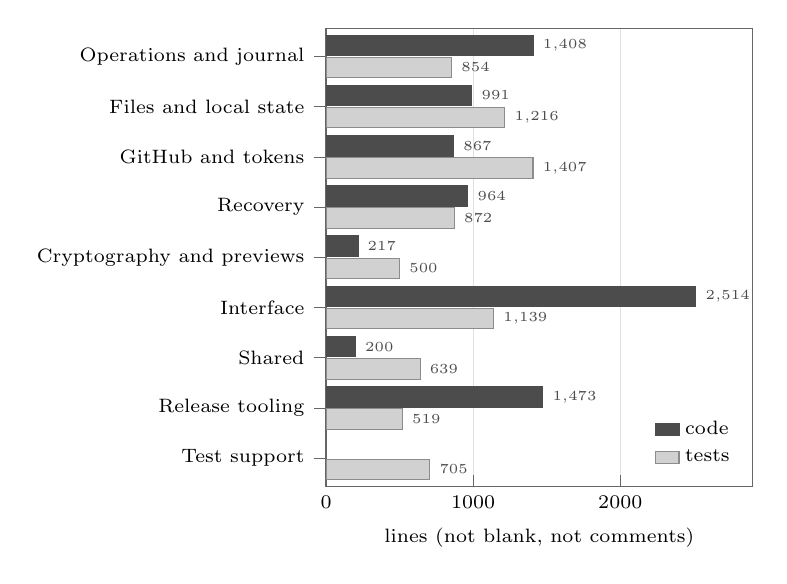
\begin{tikzpicture}
\begin{axis}[
  xbar=0.6pt, width=70mm, height=74mm,
  font=\scriptsize,
  bar width=2.6mm,
  xmin=0, xmax=2900, xtick={0,1000,2000}, xticklabels={0,1000,2000},
  scaled x ticks=false,
  xlabel={lines (not blank, not comments)},
  y dir=reverse, ytick=data, enlarge y limits=0.07,
  symbolic y coords={Operations and journal, Files and local state, GitHub and tokens, Recovery,
                     Cryptography and previews, Interface, Shared, Release tooling, Test support},
  yticklabel style={align=right},
  axis line style={black!60}, tick style={black!60},
  xmajorgrids, grid style={black!12},
  legend style={font=\scriptsize, draw=none, at={(0.98,0.02)}, anchor=south east, cells={anchor=west}},
  reverse legend,
  legend image code/.code={\draw[#1] (0mm,-0.8mm) rectangle (3mm,0.8mm);},
  xtick pos=bottom, ytick pos=left,
  nodes near coords, nodes near coords style={font=\tiny, text=black!70},
  every node near coord/.append style={anchor=west},
]
\addplot[fill=black!18, draw=black!45] coordinates {
  (854,Operations and journal) (1216,Files and local state) (1407,GitHub and tokens) (872,Recovery)
  (500,Cryptography and previews) (1139,Interface) (639,Shared) (519,Release tooling) (705,Test support)};
\addlegendentry{tests}
\addplot[fill=black!70, draw=black!70] coordinates {
  (1408,Operations and journal) (991,Files and local state) (867,GitHub and tokens) (964,Recovery)
  (217,Cryptography and previews) (2514,Interface) (200,Shared) (1473,Release tooling)};
\addlegendentry{code}
\end{axis}
\end{tikzpicture}

\caption{Lines of code per component, and of the tests assigned to the component they mainly
exercise. Counted by \code{report/data/code\_size.py}: lines that are neither blank nor comments;
docstrings count.}
\label{fig:size}
\end{figure}
